\documentclass[12pt]{article}
\usepackage{graphicx}
\usepackage{color}

\begin{document}
\begin{titlepage}
\begin{center}
\begin{huge}
\begin{center}
\textcolor{blue}{V3D Digraph Visualizer Architecture and Design}
\end{center}
\end{huge}
\hfill \break
\begin{Large}
\begin{center}
\textcolor{blue}{Team: App-Synth}
\end{center}
\end{Large}
\begin{small}
\begin{flushleft}
Author(s):
\end{flushleft}

\begin{itemize}
	\item Kulani Bamuza \\
	\item Keanan Jones \\
	\item Munyaradzi Mpofu\\
	\item Neo Thokoa\\	
	\item Takalani Sigama\\
	
\end{itemize}
\end{small}

\end{center}
\begin{center}
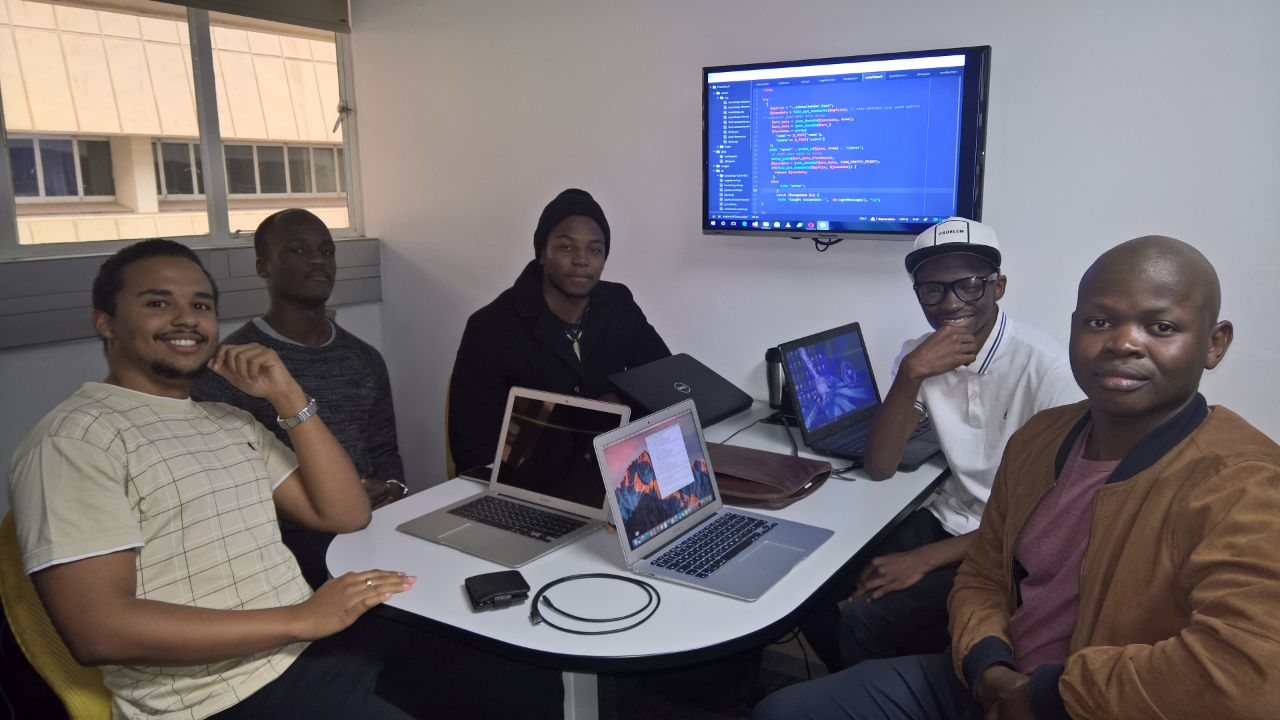
\includegraphics[scale=0.4]{Dps/TeamPic.jpg}
\\
\textcolor{blue}{\textit{University of Pretoria, Department of Computer Science
\\
15 May 2017}}

\end{center}
\end{titlepage}

\newpage
\pagenumbering{arabic}
\thispagestyle{empty}
\tableofcontents
\clearpage

\textcolor{blue}{\section{Architecture}}
\begin{flushleft}
For the V3D Digraph Visualiser, the Master-slave architecture is employed. This is due to the downstream flow of information from the "master" node(V3D app on phone) to the external display ("slave" node). \newline
All control is on the V3D mobile app, therefore this will be the master node of the system. The mobile application will stream instructions to the desktop application. 
We do this to achieve near real time synchronization between the two displays. The slave, ie. the desktop application, will receive the instructions, decode them and update the view accordingly.
\end{flushleft}

\begin{figure}[p]
\vspace*{-2.7cm}
\centering
\makebox[\linewidth]
{
	\includegraphics[width=150mm,scale=0.5]{"Deployment Diagrams/Deployment Diagram".png}
}\\[2cm]
\caption{Deployment diagram}
\end{figure}



\end{document}